\chapter{Facial Keypoints Detection}
\label{cha:Facial Keypoints Detection}

\section{Ausgangssituation}

Gesichtserkennung spielt in 21st Jahrhundert eine immer größer werdende Rolle. 
So existieren auch Herausforderungen mit den Schlüsselpunkten im Gesicht eines Menschen, welche wieder für Gesichtserkennungen verwendet werden können. 
Diese Schlüsselpunkte variieren sehr stark von Individuum zu nächsten aber auch jedes Individuum selbst hat eine Menge an Variationen. 
So spielt hier die Größe, die Position, die Neigung sowie die Beleuchtung eine Rolle und erzeugt eine fast unendliche Menge an Möglichkeiten. 
Mit Computer Vision konnten sehr viele Verbesserungen in diesem Bereich erzielt werden, wobei noch sehr viel Raum für Forschung und Verbesserungen bleibt. \newline

\noindent
Die Aufgabenstellung wird auf der Online-Plattform Kaggle \footnote{Kaggle: Facial Keypoints Detection \url{https://www.kaggle.com/c/facial-keypoints-detection}} gehostet wo auch die Trainings- und Testdaten zur Verfügung gestellt werden. 
Diese Aufgabe war im Jahr 2016 eine Herausforderung wo sich jeder beteiligen konnte, um den ersten Platz zu erreichen. 
Das Ziel für jeden Teilnehmer war es ein System zu entwickeln, welches mit den Trainingsdaten trainiert wird.
Im Anschluss sollte dieses System dann mit den Testdaten getestet werden. 
Dieses Ergebnis musste dann eingereicht werden, welches im Anschluss überprüft und bewertet wurde.

\section{Vorbereitung}

Die Daten welche zur Verfügung gestellt werden, sind auf mehreren Dateien aufgeteilt. 
In diesem Fall beinhaltet die Datei mit den Trainingsdaten die meisten Daten. 
Diese Datei beinhaltet die Bilder der Gesichter, sowie die Koordinaten der Schlüsselpunkte, gespeichert in einer CSV-Notation.
Im gesamten Gesicht gibt es 15 Schlüsselpunkte welche hier berücksichtigt werden. 
\begin{figure}[ht!]
\lstset{language=Python}
\begin{lstlisting}
left_eye_center, right_eye_center, 
left_eye_inner_corner, left_eye_outer_corner, right_eyee_inner_corner, right_eye_outer_corner, 
left_eyebrow_inner_end, left_eyebrow_outer_end, right_eyebrow_inner_end, right_eyebrow_outer_end, 
nose_tip, 
mouth_left_corner, mouth_right_corner, 
mouth_center_top_lip, mouth_center_bottom_lip
\end{lstlisting}
	\caption{$15$ Schlüsselpunkte im Gesicht eines Menschen}
	\label{fig:15keypoints}
\end{figure}
Jeder diese Schlüsselpunkte besteht aus einer X und Y Koordinate. 
Diese Datei besitzt zusätzlich in der $31$ Spalte das Bild mit dem dazugehörigen Gesicht.
Das Bild ist Encodiert abgelegt und besteht aus $96 * 96$ Werten. 
In diesem Sinne stehen nur Bilder in Graustufen zur Verfügung mit einer Auflösung von $96 * 96$ Pixel und einer Farbtiefe von $[0, 255]$, wie in der Abbildung \ref{fig:ausgangsdaten} zu erkennen ist. 
Für diese Aufgabe werde im Grunde auch nur die Konturen benötigt, was somit den einen Farbkanal erklärt aber auch die Aufgabe schwieriger macht. 
\begin{figure}
	\centering
	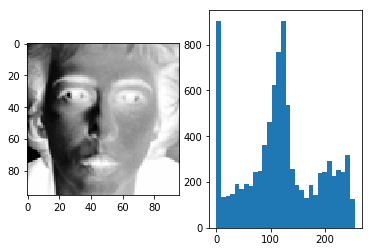
\includegraphics[scale=0.8]{images/ausgangsDaten.png}
	\caption{Ein Gesicht aus dem Datenbestand mit der Verteilung der Graustufenwerten}
	\label{fig:ausgangsdaten}
\end{figure}
\begin{figure}[ht!]
\lstset{language=Python}
	\begin{lstlisting}
# left\_eye\_center, right\_eye\_center
66.0335639098,39.0022736842,30.2270075188,36.4216781955
# left\_eye\_inner\_corner, left\_eye\_outer\_corner
59.582075188,39.6474225564,73.1303458647,39.9699969925
# right\_eye\_inner\_corner, right\_eye\_outer\_corner
36.3565714286,37.3894015038,23.4528721805,37.3894015038
# left\_eyebrow\_inner\_end, left\_eyebrow\_outer\_end
56.9532631579,29.0336481203,80.2271278195,32.2281383459
# right\_eyebrow\_inner\_end, right\_eyebrow\_outer\_end
40.2276090226,29.0023218045,16.3563789474,29.6474706767
# nose\_tip
44.4205714286,57.0668030075
# mouth\_left\_corner, mouth\_right\_corner
61.1953082707,79.9701654135,28.6144962406,77.3889924812
# mouth\_center\_top\_lip, mouth\_center\_bottom\_lip
43.3126015038,72.9354586466,43.1307067669,84.4857744361
# image
238 236 237 238 240 240 239 241 241 243 240 239 231 212 ...
\end{lstlisting}
	\caption{Ein gesamter Datensatz aus den Trainingsdaten mit den X und Y Werten pro Schlüsselpunkt}
	\label{fig:ausgangsdatenRoh}
\end{figure}

\subsection{Daten vorbereiten und normalisieren}

Diese Daten müssen zu Beginn vorbereitet und normalisiert werden. 
Um Problemgröße zu verringern empfiehlt es sich die Aufgabe aufzuteilen auf mehrere Netzwerke. 
Dies hat einen zusätzlichen Grund, da die Trainingsdaten nicht komplett sind und somit nicht zu allen Bildern alle 15 Schlüsselpunkte vorhanden sind. 
Sollte dies ignoriert werden, würde sich die Anzahl der zur Verfügung stehenden Datensätze von $7049$ auf $2140$ reduzieren. 
Ein weiterer Grund für die Auftrennung der Problemstellung ist, da Ressourcen leichter verteilt werden können und die Netzwerke noch fein angepasst werden könnten. \newline

\noindent
Unter der Zuname von Pandas \footnote{Pandas: Python Data Analysis Library \url{http://pandas.pydata.org/}} und NumPy \footnote{NumPy: Scientific Computing \url{http://www.numpy.org/}} besteht die Möglichkeit sehr einfach und Effizient auf die Datensätze zuzugreifen und diese zu Verwenden. 
Wie in der Codebeispiel \ref{fig:datenLesenEinschränken} ersichtlich ist, werden die Daten mit Hilfe von Pandas geladen und unter Zunahme von NumPy normalisiert und neu strukturiert. 
\begin{figure}[ht!]
\lstset{language=Python}
\begin{lstlisting}
import pandas as pd
import numpy as np

# konstanten Definition
IMAGE_SIZE = 96

# Daten einlesen
df = pd.read_csv('~/training.csv')

# Bilder um konvertieren in eine List von Zahlen
df['Image'] = df['Image'].apply(lambda im: np.fromstring(im, sep=' '))

# die Aktuell benötigten Spalten herausnehmen
df = df[['left_eye_center', 'right_eye_center', 'Image']]

# entfernen unvollständiger Datensätze
# Verkleinerung der Datensätze von 7049 auf 7033
df = df.dropna()

# normalisieren der Bilder in einen Wertebereich von [0, 1] 
# und überführen in eine 96 mal 96 Matrix
# Variable X beinhaltet alle Bilder des Datensatzes welche Vollständig sind
X = np.vstack(df['Image']) / 255.
X = X.reshape(-1, IMAGE_SIZE, IMAGE_SIZE, 1)

# explizites definieren des Datentyps für die Werte das Bild
X = X.astype(np.float32)

# normalize the X, Y Koordinaten in einen Wertebereich von [0, 1]
# Variable Y beinhaltet die Labels zu allen Bildern
Y = df[df.columns[:-1]].values
Y = Y / 96.0
\end{lstlisting}
	\caption{Daten einlesen und einschränken}
	\label{fig:datenLesenEinschränken}
\end{figure}

\subsection{Evaluation- und Errorfunktion}

Die Ergebnisse des Netzwerkes müssen in jedem Fall, im Bereich des maschinellen Lernens in der überwachten Form, verglichen und Validiert werden. 
In diesem Beispiel handelt es sich nicht um eine Klassifizierungsaufgabe, sondern um eine Regressionsproblemstellung. 
In diesem Fall kann nicht eine einfach 'Cross Entroy' \textbf{TODO checken} Funktionen verwendet werden, um die Daten zu evaluieren und zu adaptieren. 
Aus diesem Grund muss dies Manuel durchgeführt werden und selbst eine Berechnung aufgestellt werden, welche diese Werte liefert, damit diese einem Optimierer übergeben werden können. 
Der Verlust beziehungsweise die Differenz zwischen Ergebnis des Netzwerkes und dem bekannten Ergebnis, kann durch eine Subtraktion sowie einer Quadrierung berechnet werden. 
Diese ist in der Gleichung \ref{eq:lossCalc} zu erkennen, wobei \textit{graph} eine Matrix (Tensor) an Ergebnissen ist, mit der Anzahl an Zeilen wie in der Konstante \textit{BATCH\_SIZE} definiert. 
Die Variable \textit{train\_labels\_node} beinhaltet die bekannten Ergebnisse zu Bilder mit den selben Dimensionen wie in der Matrix \textit{graph}. 
\textit{tf.subtract} führt eine Subtraktion auf jeden Inhalt der beiden Matrizen aus, was auch dazu führt, dass diese die selben Dimensionen haben müssen. 
\textit{tf.square} quadriert die berechneten Differenzen um negative Werte zu entfernen. 
Zum Abschluss werden alle Ergebnisse in der Ergebnismatrix mit \textit{tf.reduce\_sum} aufsummiert, was zu einem Skalarenergebnis führt. 
Für diese konkrete Implementierung wurde als Opitmierungsalgorithmus ein \textit{Adam}-Algorithmus \textbf{TODO Adam} verwendet. 
Um das Verlustergebnis für einen Leser lesbare zu machen, muss der Verlustwert durch die Anzahl der Batchgröße dividiert werden, was die Differenz in einem Datensatz als Durchschnitt ergibt. 
Die gesamte Umsetzung ist im Codebeispiel \ref{fig:VerlustKonkreOpitimier} zu finden. 
\begin{equation}
	Verlust := \sum{(R - L)^2}
	\label{eq:lossCalc}
\end{equation}
\begin{figure}[ht!]
\lstset{language=Python}
\begin{lstlisting}
import tensorflow as tf

# konstanten Definition
BATCH_SIZE = 64

# Verlustberechnung
with tf.name_scope("loss"):
    # sollte sich im Laufe der Trainingsphasen an 0 annähern
    loss = tf.reduce_sum(
    			tf.square(
    				tf.subtract(graph, train_labels_node)
    			)
    		)

# Auswahl eines konkreten Optimierungsalgorithmuses in der Kurzschreibweise
# mit einer Lernrate von 0.00001
with tf.name_scope("train"):
    train = tf.train.AdamOptimizer(learning_rate=1e-5).minimize(loss)
    
# Verlustwert durch die Anzahl der Bilder im Batch da diese Werte 
# zusammen Summiert werden
with tf.name_scope("accuracy"):    
    accuracy = loss / BATCH_SIZE
\end{lstlisting}
	\caption{Verlustberechnung, konkreter Opitimierungsalgorithmus, Genauigkeitberechnung}
	\label{fig:VerlustKonkreOpitimier}
\end{figure}
 
\section{Neuronale Ebenen vorbereiten}

Damit die Ebenen einfacher verwendet werden können, können dies als konfigurierbare Muster definiert werden. 
Dadurch wird erzielt, dass gleiche Ebenen im visualisierten Graphen die selbe Farbe besitzen und zum anderen alle Inhalte darin zusammengefasst werden. 
Im Grunde existieren zwei verschieden Haupttypen an Ebenen. 
Zum einen die Convolutional-Ebenen und zum anderen die Vollvernetzen-Ebenen. 
Wie im Code \ref{fig:ConvFc} ersichtlich ist besitzen beide Hauptgruppen an Ebenen jeweils eine Datenquelle beschrieben als \textit{x\_} und Gewichtungen und Biaseswerte. 
Die Bias Werte werden dabei immer erst nach der Kernfunktion an das Ergebnis angefügt und somit in der Aktivierungsfunktion berücksichtigt. 
\begin{figure}[ht!]
\lstset{language=Python}
\begin{lstlisting}
def conv_layer(x_, size_in, size_out, name="conv"):
    with tf.name_scope(name):
        weights = tf.Variable(tf.truncated_normal([3, 3, size_in, size_out], dtype=tf.float32, stddev=1e-1), 
                              trainable=True, name='weights')
        conv = tf.nn.conv2d(x_, weights, [1, 1, 1, 1], padding='SAME')
        biases = tf.Variable(tf.constant(0.0, shape=[size_out], dtype=tf.float32), 
                             trainable=True, name='biases')
        bias = tf.nn.bias_add(conv, biases)
        conv = tf.nn.relu(bias, name="act")

    maxPool = tf.nn.max_pool(conv, 
                             ksize=[1, 2, 2, 1],
                             strides=[1, 2, 2, 1],
                             padding='VALID')

    return conv

def fc_layer(x_, size_out, name="fc", act=None):
    with tf.name_scope(name):
        size_in = x_.get_shape()[1].value
        weights = tf.Variable(tf.truncated_normal([size_in, size_out], dtype=tf.float32, stddev=1e-2), 
                              trainable=True, name='weights')
        biases = tf.Variable(tf.constant(0.0, shape=[size_out], dtype=tf.float32), 
                                  trainable=True, name='biases')
        mul = tf.nn.xw_plus_b(x_, weights, biases)
        
        if act is not None:
            mul = act(mul)

        return mul
\end{lstlisting}
	\caption{Definition der Convolutional- und Vollvernetzen-Ebenen}
	\label{fig:ConvFc}
\end{figure}

\section{Neuronale Ebenen verknüpfen}

Diese Definitionen der Ebenen aus dem Codefragment \ref{fig:ConvFc} müssen nun in einem Netzwerk zusammen vernetzt werden. 
Ein neuronales Netzwerk welches relative leichtgewichtig ist und diese Problematik relative brauchbar lösen kann, ist im Grunde ein sehr vereinfachtes 'VGG16' Netzwerk \footcite{VGG16: TODO}.
Für diesen Fall besteht dieses aus $3$ Convolutional-Ebenen und $3$ Vollvernetzen-Ebenen, wie im Codefragment \ref{fig:buildGraph} zu sehen ist. 
Das originale VGG16 Netzwerk besitzt im Gegensatz zu aktuell verwendeten, $5$ Convolutional-Ebenen mit je $2$ integrierten Convolutional-Ebenen mit den selben Dimensionen und die Hauptebenen $3, 4, 5$ sogar $3$ Convolutional-Ebenen. 
Die letzte Ebene der Vollvernetzen-Ebenen wird dabei ohne Aktivierungsfunktion ausgeführt, um die Roh-Ergebnisse zu bekommen. 
Im aktuellen Fall werden für die $2$ Iris-Positionen im Gesicht $4$ Ergebnisse benötigt. 
\begin{figure}[ht!]
\lstset{language=Python}
\begin{lstlisting}
def model(data):
    net = conv_layer(data, 1, 32, "conv1")
    net = conv_layer(net, 32, 64, "conv2")
    net = conv_layer(net, 64, 128, "conv3")

	# Transformieren in eine flache Struktur
    dims = net.get_shape()[1:]
    k = dims.num_elements()
    with tf.name_scope('flatten'):
        net = tf.reshape(net, [-1, k])
    
    net = fc_layer(net, 256, "fc1", tf.nn.relu)    
    net = fc_layer(net, 256, "fc2", tf.nn.relu)
    net = fc_layer(net, 4, "fc3")
    
    return net
    
# Definition der Platzhalter für die Datenübergabe
train_data_node = tf.placeholder(tf.float32, shape=(BATCH_SIZE, IMAGE_SIZE, IMAGE_SIZE, 1))
train_labels_node = tf.placeholder(tf.float32, shape=(BATCH_SIZE, 4))

# erstellen eines Graphen mit dem definierten Model
graph = model(train_data_node)
\end{lstlisting}
	\caption{Modeldefinition des Graphen}
	\label{fig:buildGraph}
\end{figure}

\section{Trainieren}

Um das erzeugte Netzwerk aus \ref{fig:buildGraph} verwenden und trainieren zu können, muss dieses zu erst Initialisiert werden. 
Wie im Code \ref{fig:initRun} zu erkennen ist wird ein globale Initialisierung verwendet welchen alle Konstanten und Variablen der aktuellen Umgebung initialisiert. 
In der For-Schleife werden fast alle Datensätze einmal durch den Graphen gesendet und entweder zum Trainieren oder Evaluieren verarbeitet. 
Der Session wird in der \textit{Run}-Methode eine Liste and Endpunkten des Graphen mitgegeben welche Evaluiert werden sollen. 
In der Trainingsphase ist dies der Optimierungsendpunkt und in der Evaluierungsphase die Punkte \textit{accuracy} und \textit{graph}. 
Accuracy damit ein vergleichbarer Wert zur Verfügung steht, an welchem der Lernfortschritt erkennbar ist und der Hauptendpunkt des Graphen selbst, damit die Ergebnis direkt in die Bilder gezeichnet werden können. 
Dies ermöglicht eine visualisierte Verifikation durch einen Supervisor. 
\begin{figure}[ht!]
\lstset{language=Python}
\begin{lstlisting}
# erstellen einer Session
sess = tf.Session()

# erstellen einer globalen Initialisierungsroutine
init_op = tf.global_variables_initializer()
# initialisieren aller Konstanten und Variablen
sess.run(init_op)

# durchlaufen aller Datensätze
runing = train_data.shape[0] // BATCH_SIZE
for i in range(runing):
    offset = i * BATCH_SIZE
    
    # laden eines Datenbatches aus den Datensätzen
    batch_data = train_data[offset:(offset + BATCH_SIZE), ...]
    batch_labels = train_labels[offset:(offset + BATCH_SIZE)]
    
    # ersetzen der Platzhalter durch die konkreten Daten
    feed = {train_data_node: batch_data, 
            train_labels_node: batch_labels}
     
    # ausführen des Graphen zur Evaluierung
    if i % 5 == 0:
        [train_accuracy, data] = sess.run([accuracy, graph], feed_dict=feed)
        print data[0:4]
        print batch_labels[0:4]
        
        print i, train_accuracy
        
    # ausführen einer Trainingsiteration
    else:
        sess.run(train, feed_dict=feed)
\end{lstlisting}
	\caption{Initialisierung des Graphen und durchführen einer Epoche}
	\label{fig:initRun}
\end{figure}

\section{Validierungsresultate}






